\documentclass[runningheads]{llncs}

\usepackage{natbib}

\usepackage[T1]{fontenc}

\usepackage{amsfonts}

\usepackage{amsmath}

\usepackage{graphicx}

\usepackage{svg}

\usepackage{acronym}

\usepackage{hyperref}

\usepackage{subfig}



\newcommand{\topic}{Approaches for finding sample pairs in contrastive learning}
\newcommand{\authorA}{Klara M. Gutekunst}

% If you use the hyperref package, please uncomment the following two lines
% to display URLs in blue roman font according to Springer's eBook style:
%\usepackage{color}
%\renewcommand\UrlFont{\color{blue}\rmfamily}
%\urlstyle{rm}
%
\begin{document}

%
\title{\topic}
%
\titlerunning{\topic}

\author{\authorA}
%
\authorrunning{\authorA}

\institute{University of Kassel, Germany\\
\email{klara.gutekunst@student.uni-kassel.de}}
%
\maketitle         
%
% include: speed bonus, no reloads, but no nesting, forces page break after and before input
\begin{abstract}
    %The abstract should briefly summarize the contents of the paper in
    %150--250 words.

    Unsupervised learning techniques are of interest to many researchers, as they allow training models on data without any labels.
    \ac{ssl} is a subset of unsupervised learning, where labels are generated from unlabelled training data.
    \ac{cl} is a \ac{ssl} technique that is frequently used in representation learning.
    The representations of similar samples are supposed to be encoded within close range of each other, 
    while the representations of dissimilar samples are pushed apart.
    The selection of these dis-/similar pairs is subject to research.
    This paper reviews different approaches for finding sample pairs in \ac{cl}, with a focus on hard sample mining.
    
    \keywords{\acl{cl}  \and \acl{ssl} \and Hard sample mining.}
    \end{abstract}

\section{Introduction}\label{sec:introduction}

\acf{ssl} is an unsupervised learning technique that allows training models on data without any labels.
The idea is to generate labels from the unlabelled training data contemplating a pre-text task.

Researchers usually select self-supervised pre-text tasks such that 
the targets can be generated without human annotations \citet{PIC_2020}.
The pre-text instance discrimination task considers each instance from the dataset its class.
A sample and its augmentations are considered positive pairs, 
while all other samples are considered negative pairs.
Hence, the model acquires an understanding of distinguishing between the instances and 
learns invariance to (image) transformations \citet{PIC_2020,swav_2020,local_aggr_2019,grape_2024,wang_understanding_2021}.

In order to explain why the proximity of generated samples to the anchor is relevant to the efficiency during training, 
one can consider a simple example in Euclidean space.
Imagine images as input to a \ac{nn}, which projects them onto $f_{\theta}(x) \in \mathbb{R}^d$, where $theta$ are the parameters of the \ac{nn}.

\begin{figure}[htbp]
    \centering
    \includesvg[width=300pt]{images/Hard_easy_samples_dist_effect_loss}
    \caption{svg image}
\end{figure}

% main part



The selection of positive pairs ($x$, $x^+$) is subject to multiple papers, 
which propose different strategies.
In the case of unsupervised learning, generally, 
the positive sample $x^+$ is generated by applying a transformation to the anchor $x$.
Popular augmentation techniques include random cropping, color jittering, 
rotation and scaling \citet{ho_contrastive_2020,robinson_contrastive_2021}.

% PU learning
Another approach is to use so-called \ac{pu} learning, where learning is carried out 
on a set of positive and a set of unlabeled samples \citet{chuang_debiased_2020}.

% unsupervised learning
Simple selection techniques of negative samples include uniform sampling from the dataset or batch.
However, this approach is prone to two issues \citet{robinson_contrastive_2021,mining_potential_2024}:
\begin{enumerate}
    \item Selected samples are not necessarily hard negatives since the approach does not consider the embedding space proximity.
    \item Selected samples might actually belong to the same class as the anchor and thus, can be denoted \ac{fn}.
\end{enumerate}

% oracle learning
Some approaches use a so-called class oracle to boost the performance of the model.
If \acp{fn} \cite{grape_2024,curricular_weighting_2024,progcl_2022}, i.e. 
samples that belong to the latent class of the anchor but are considered negative, 
are sampled during hard negative mining, 
samples of the same class are pushed further apart in the embedding space. 
To avoid performance deterioration, this approach removes the \acp{fn} from the set of negative samples and thus, 
increases the performance of the model \citet{mochi_2020}.

\section{Related Work}\label{sec:related_work}

% sampling from distributions
Naturally, when using descriptive statistics to describe data, (empirical estimated) distributions play a crucial role.
Some researchers obtain their positive and negative samples from distributions.
Unfortunately, since \ac{cl} is a form of unsupervised learning, 
the true data distribution of the different classes is often not available.
Therefore, some scientists formulate assumptions or simplify the problem.
Possible assumptions include that the data distribution is uniform,
or approximating the positive sample distribution by sampling from a set of transformations 
or using the overall data distribution as a proxy for the negative sample distribution \citet{chuang_debiased_2020,robinson_contrastive_2021}.
In other cases, the class distributions are approximated using \acp{bmm} \citet{progcl_2022}.

Given the assumption that the data distribution is sufficiently well approximated, 
it is possible to consider probabilities of samples being \acp{fn} during the selection process of samples.
Needless to say, the goal is to avoid sampling \acp{fn} as negative samples.
To this end, scientists have proposed different strategies, which mostly boil down to 
incorporating the possibility of a potential negative sample being a \ac{fn} or \ac{tn} 
\citet{chuang_debiased_2020,robinson_contrastive_2021,progcl_2022}.


% augmentation strategies
Irrespective of its usage in the context of estimation of distributions, 
data augmentation is a common technique to create positive samples.
Often, an augmentation strategy is randomly sampled from a set of possible augmentations.
The motivation behind this is to increase the diversity of the positive samples 
in order to drive the model to learn features invariant to translations 
\citet{PIC_2020,swav_2020,local_aggr_2019,grape_2024,CL_temp_2021}.


% clustering/ distance
Since \ac{cl} objectives are often formulated in terms of distances or similarities between pairs of samples, 
the idea of using clustering techniques is a natural choice.
Intuitively, clusters of similar samples should be considered as positive samples and thus,
should be encoded close to each other.
Conversely, samples from different clusters should be encoded far apart.

Multiple methods have been proposed to generate samples via clustering.
Some ideas focus on high intra-cluster similarities to improve the alignment of the embeddings \citet{DRC_2020}.
Other ideas define different neighbour regions to condense representation within an inner radius 
while repelling samples from an outer radius \citet{local_aggr_2019}.
Another approach is to consider both Euclidean distance and semantic similarity to generate hard samples \citet{mining_manifolds_2018}.
Moreover, the \ac{pcl} technique defines positive samples as cluster centroids 
from one of the multiple clusterings for different numbers of clusters 
to encode the hierarchical structure of the data \citet{PCL_2021}.


% memory bank
Another prominent concept is the usage of memory banks to store embeddings of the data.
\citet{mochi_2020} fill these memory banks with embeddings of negative samples 
and propose two approaches for generating new hard negatives: 
Two of the most difficult samples currently stored in the memory bank are randomly selected and mixed.
The second approach is to use only one of the existing negative samples and 
mix it with the anchor to create a new sample.

\citet{progcl_2022} propose a method that extends the idea of \citet{mochi_2020} by weighting randomly selected negative samples 
with their relative similarity to the anchor when mixing them to create more difficult negative samples.

It is also possible to use the memory bank to store the embeddings of the positive samples.
Similarly, either randomly chosen samples can be used individually or 
the samples can be weighted by their hardness during loss calculation \citet{mining_potential_2024}.


% other work
% EM-algorithm
Multiple approaches, including \ac{drc}, \ac{pcl} and \progcl{}, use the \ac{em} algorithm 
to reduce computational costs or to find solutions via approximations.
Both \ac{drc} \citet{DRC_2020} and \progcl{} \citet{PCL_2021} are clustering-based methods 
while \progcl{} \citet{progcl_2022} is a distribution-based method.

% temperature
Since most approaches use a temperature parameter to control the hardness of the negative samples, 
\citet{CL_temp_2021} and \citet{grape_2024} investigate the impact of the temperature on the performance of the model.
They find that the \ac{cl} loss function optimizes hard samples by penalizing them according to their hardness.
If the temperature is small, only the closest points are penalized and others are not.
This can result in a uniformly distributed embedding space.

% curriculum learning
\citet{curricular_weighting_2024} propose a curriculum learning approach to generate hard negative samples.
They outline why curriculum learning is beneficial for \ac{cl} and how it can be implemented.

% data scheduling
% \citet{PIC_2020} propose a method to schedule the data for training 
% to reduce the periods within which a sample is not considered for training.

\section{Sampling techniques}\label{sec:sampling_techniques}

Since positive pairs ($x$, $x^+$) are considered to originate from the same class, we denote $\rho(c), c \in \mathcal{C}$ as the distribution over the latent classes.
Moreover, let $h: \mathcal{X} \rightarrow \mathcal{C}$ be the ground truth assigning class labels $c \in \mathcal{C}$ to inputs $x \in \mathcal{X}$.
Hence, $x \sim x'$ if $h(x) = h(x')$ \citet{robinson_contrastive_2021,chuang_debiased_2020}.
Assuming that $\rho(c)$ is uniformly distributed, and that $x^- \sim q = p$ where the anchor $x$ 
is drawn from the data distribution $p$.

\subsection{Robinson's Hard Negatives}\label{subsec:robinson_hard_negatives}

Since positive pairs ($x$, $x^+$) are considered to originate from the same class, we denote $\rho(c), c \in \mathcal{C}$ as the distribution over the latent classes.
Moreover, let $h: \mathcal{X} \rightarrow \mathcal{C}$ be the ground truth assigning class labels $c \in \mathcal{C}$ to inputs $x \in \mathcal{X}$.
Hence, $x \sim x'$ if $h(x) = h(x')$.
Assuming that $\rho(c)$ is uniformly distributed, and that $x^- \sim q = p$ where the anchor $x$ 
is drawn from the data distribution $p$, \citet{robinson_contrastive_2021} 
propose a novel approach to sample hard negatives from $q \neq p$.

This method balances both the risk of sampling \ac{fn} and the degree of hardness of the samples obtained.
Moreover, via the concentration parameter $\beta$, the user can decide how hard the negatives should be and thus, how likely they have the same target as the anchor.
Large values of $\beta$ lead to sampling very hard negative samples.
The authors of \citet{robinson_contrastive_2021} propose negative samples from $q^-_{\beta}(x^-)$, 
which enforces $x$, $x^-$ having different classes by conditioning on dissimilar classes.
By computing a scalar product of both representations $f(x)$, $f(x^-)$ in \eqref{eq:q_beta}, 
they encourage similar represented samples.
Unfortunately, it is unclear how to sample from $q^-_{\beta}(x^-)$ and thus, 
the authors propose a way to rewrite the equation to facilitate sampling.

\begin{align} 
    q^-_{\beta}(x^-) = q_\beta(x^-|h(x) \neq h(x^-)) \propto \exp(\beta f(x)^\text{T}f(x^-))\cdot p(x^-) 
\label{eq:q_beta}
\end{align} 


Since sampling could both yield \ac{fn} and \ac{tn}, it is possible to rewrite \eqref{eq:q_beta_minus} 
displaying both cases in \eqref{eq:fn_tn}.
The first term corresponds to the probability of sampling \ac{tn}, i.e. $h(x) \neq h(x')$,
 while the second term corresponds to the probability of sampling \ac{fn} with $x \sim x'$.

 \begin{align}
    q_\beta(x^-) &= \rho(c)q^{-}_\beta(x^-) + (1-\rho(c))q^{+}_\beta(x^-)
    \label{eq:fn_tn}
\end{align}

The distribution $q^{+}_\beta(x^-)$ can described in more detail.
Given that $x$ and $x^-$ are from the same class, 
the probability of sampling $x^-$ is proportional to the exponential of the scalar product of the 
representations of $x$ and $x^-$ as described in \eqref{eq:q_beta_plus}.

\begin{align}
    q^{+}_\beta(x^-) &= q_\beta(x^-|h(x) = h(x^-)) &\propto \exp(\beta f(x)^\text{T}f(x^-))\cdot p^+(x^-) 
    \label{eq:q_beta_plus}
\end{align}

Finally, we can rewrite \eqref{eq:fn_tn} to obtain the desired distribution $q^-_{\beta}(x^-)$ as shown in \eqref{eq:q_beta_minus}.
This version of the distribution allows for sampling from $q^-_{\beta}(x^-)$, since we can sample from $q_\beta(x^-) \approx p$ 
and we can approximate $q^{+}_\beta(x^-)$ by sampling from a set of transformations.    % rejection sampling & Monte Carlo sampling

\begin{align}
    q^{-}_\beta(x^-) &= \frac{(q_\beta(x^-)-(1-\rho(c))q^{+}_\beta(x^-))}{\rho(c)} 
    \label{eq:q_beta_minus}
\end{align}



% \begin{align*}
%     q^{-}_\beta(x^-) &=  q_\beta(x^-|h(x) \neq h(x^-)) 
% &\propto \exp(\beta f(x)^\text{T}f(x^-))\cdot p(x^-) 
% \\&= \rho(c)q^{-}_\beta(x^-) + (1-\rho(c))q^{+}_\beta(x^-)
% \\&= \rho(c)\frac{(q_\beta(x^-)-(1-\rho(c))q^{+}_\beta(x^-))}{\rho(c)} + (1-\rho(c))q_\beta(x^-|h(x) = h(x^-)) &\propto \rho(c)q^{-}_\beta(x^-) + \exp(\beta f(x)^\text{T}f(x^-))\cdot p^+(x^-) 
% \end{align*}

\subsection{Adversarial Examples}\label{subsec:adversarial_examples}
% idea of positive pair: fix one augmented sample (randomly) and choose most diverse adversarial perturbation for other sample

\citeauthor{ho_contrastive_2020} propose the \ac{clae} method to generate adversarial examples 
(both negative and positive) attacking the network and thus,
can be considered the most challenging examples \cite{ho_contrastive_2020}.
Adversarial attacks will induce a network in error.
Adversarial training includes both clean and adversarial examples in the training set to defend against those attacks and 
increase the network's robustness.
However, according to \citeauthor{ho_contrastive_2020}, the aim is not to enhance robustness to attacks 
but to improve the representation of the network.

\ac{clae} produces both positive and negative samples from the batch.
Adversarial examples are generated from clean examples $x$.
The authors want to select the optimal transformations $p_i, q_i \in \mathcal{T}$ for each sample $x_i$ in the batch.
Optimal transformations are those that maximize the loss function $L_{cl}$.
Since it is difficult to find two optimal transformations simultaneously, 
\citeauthor{ho_contrastive_2020} propose fixing one transformation $q_i$ and 
optimizing the other $p_i$ as defined in \eqref{eq:clae_optimal_transformations}.
$q_i$ is sampled randomly from the set of transformations $\mathcal{T}$.

\begin{equation}
    \left\{p^*_i\right\} = \arg\max_{\left\{p_i\right\} \in \mathcal{T}} \sum_{i}^{}L_{cl}(x_i^{p_i}, x_i^{q_i}; \theta, \mathcal{T}), q^*_i \sim \mathcal{T}
    \label{eq:clae_optimal_transformations}
\end{equation}

Due to the inefficiency of a complete search over $\mathcal{T}$, 
the authors propose directly choosing an adversarial perturbation $x^{r_i}_i$ of the fixed augmentation $x_i^{q_i}$.
Hence, they choose the perturbation $x^{r_i}_i = x^{q_i}_i + \delta^*_i$ from 
$A(x^{q_i}_i) = \left\{x' | x' = x^{q_i}_i + \delta, \left\|\delta\right\|_p < \epsilon\right\}$,
which leads to the most diverse positive pair ($x^{r_i}_i$, $x^{q_i}_i$).

The mathematical details of obtaining $x^{r_i}_i$ are provided in \citet{ho_contrastive_2020}.
The idea is that the loss function enforces 
positive pair representations $f(x^{r_i}_i)$ and $f(x^{q_i}_i)$ to be close to each other,
while representations of perturbations of different examples $f(x^{p_k}_k)$ and $f(x^{q_i}_i)$ are separated.

Generally, any set of transformations $\mathcal{T}$ can be used to generate adversarial examples.
\citeauthor{ho_contrastive_2020} use the \ac{fgsm} method which 
produces adversarial augmentations in consideration of the whole batch.

It is important to note that the usage of adversarial samples in training may result in 
the degradation of the downstream classification accuracy.

\subsection{Debiased Contrastive Learning}\label{subsec:debiasing_cl}

\citet{chuang_debiased_2020} propose a debiased contrastive objective that corrects for sampling \acp{fn}, 
i.e., the selection of negative samples that have the same label as the anchor, in an unsupervised scenario.
They denote sampling bias the phenomenon where anchor $x$ and negative sample $x^-$ are similar to each other.
When randomly sampling negative samples from the data distribution $p(x)$ 
a negative sample can inherently belong to the same latent class as the anchor.
This phenomenon is illustrated in \autoref{fig:sampling_bias}a.
The effect of sampling bias on the model's performance is illustrated in \autoref{fig:sampling_bias}b.

\begin{figure}%
    \centering
    \subfloat[\centering Visualization of sampling bias similar to \citet{chuang_debiased_2020}. Sampling $x_i^-$ from $p$ can result in \ac{fn}.]
    {{\includegraphics[width=5cm]{images/sampling_bias.png} }}%
    \qquad
    \subfloat[\centering Negative influence of sampling bias on accuracy from \citet{chuang_debiased_2020}.]{{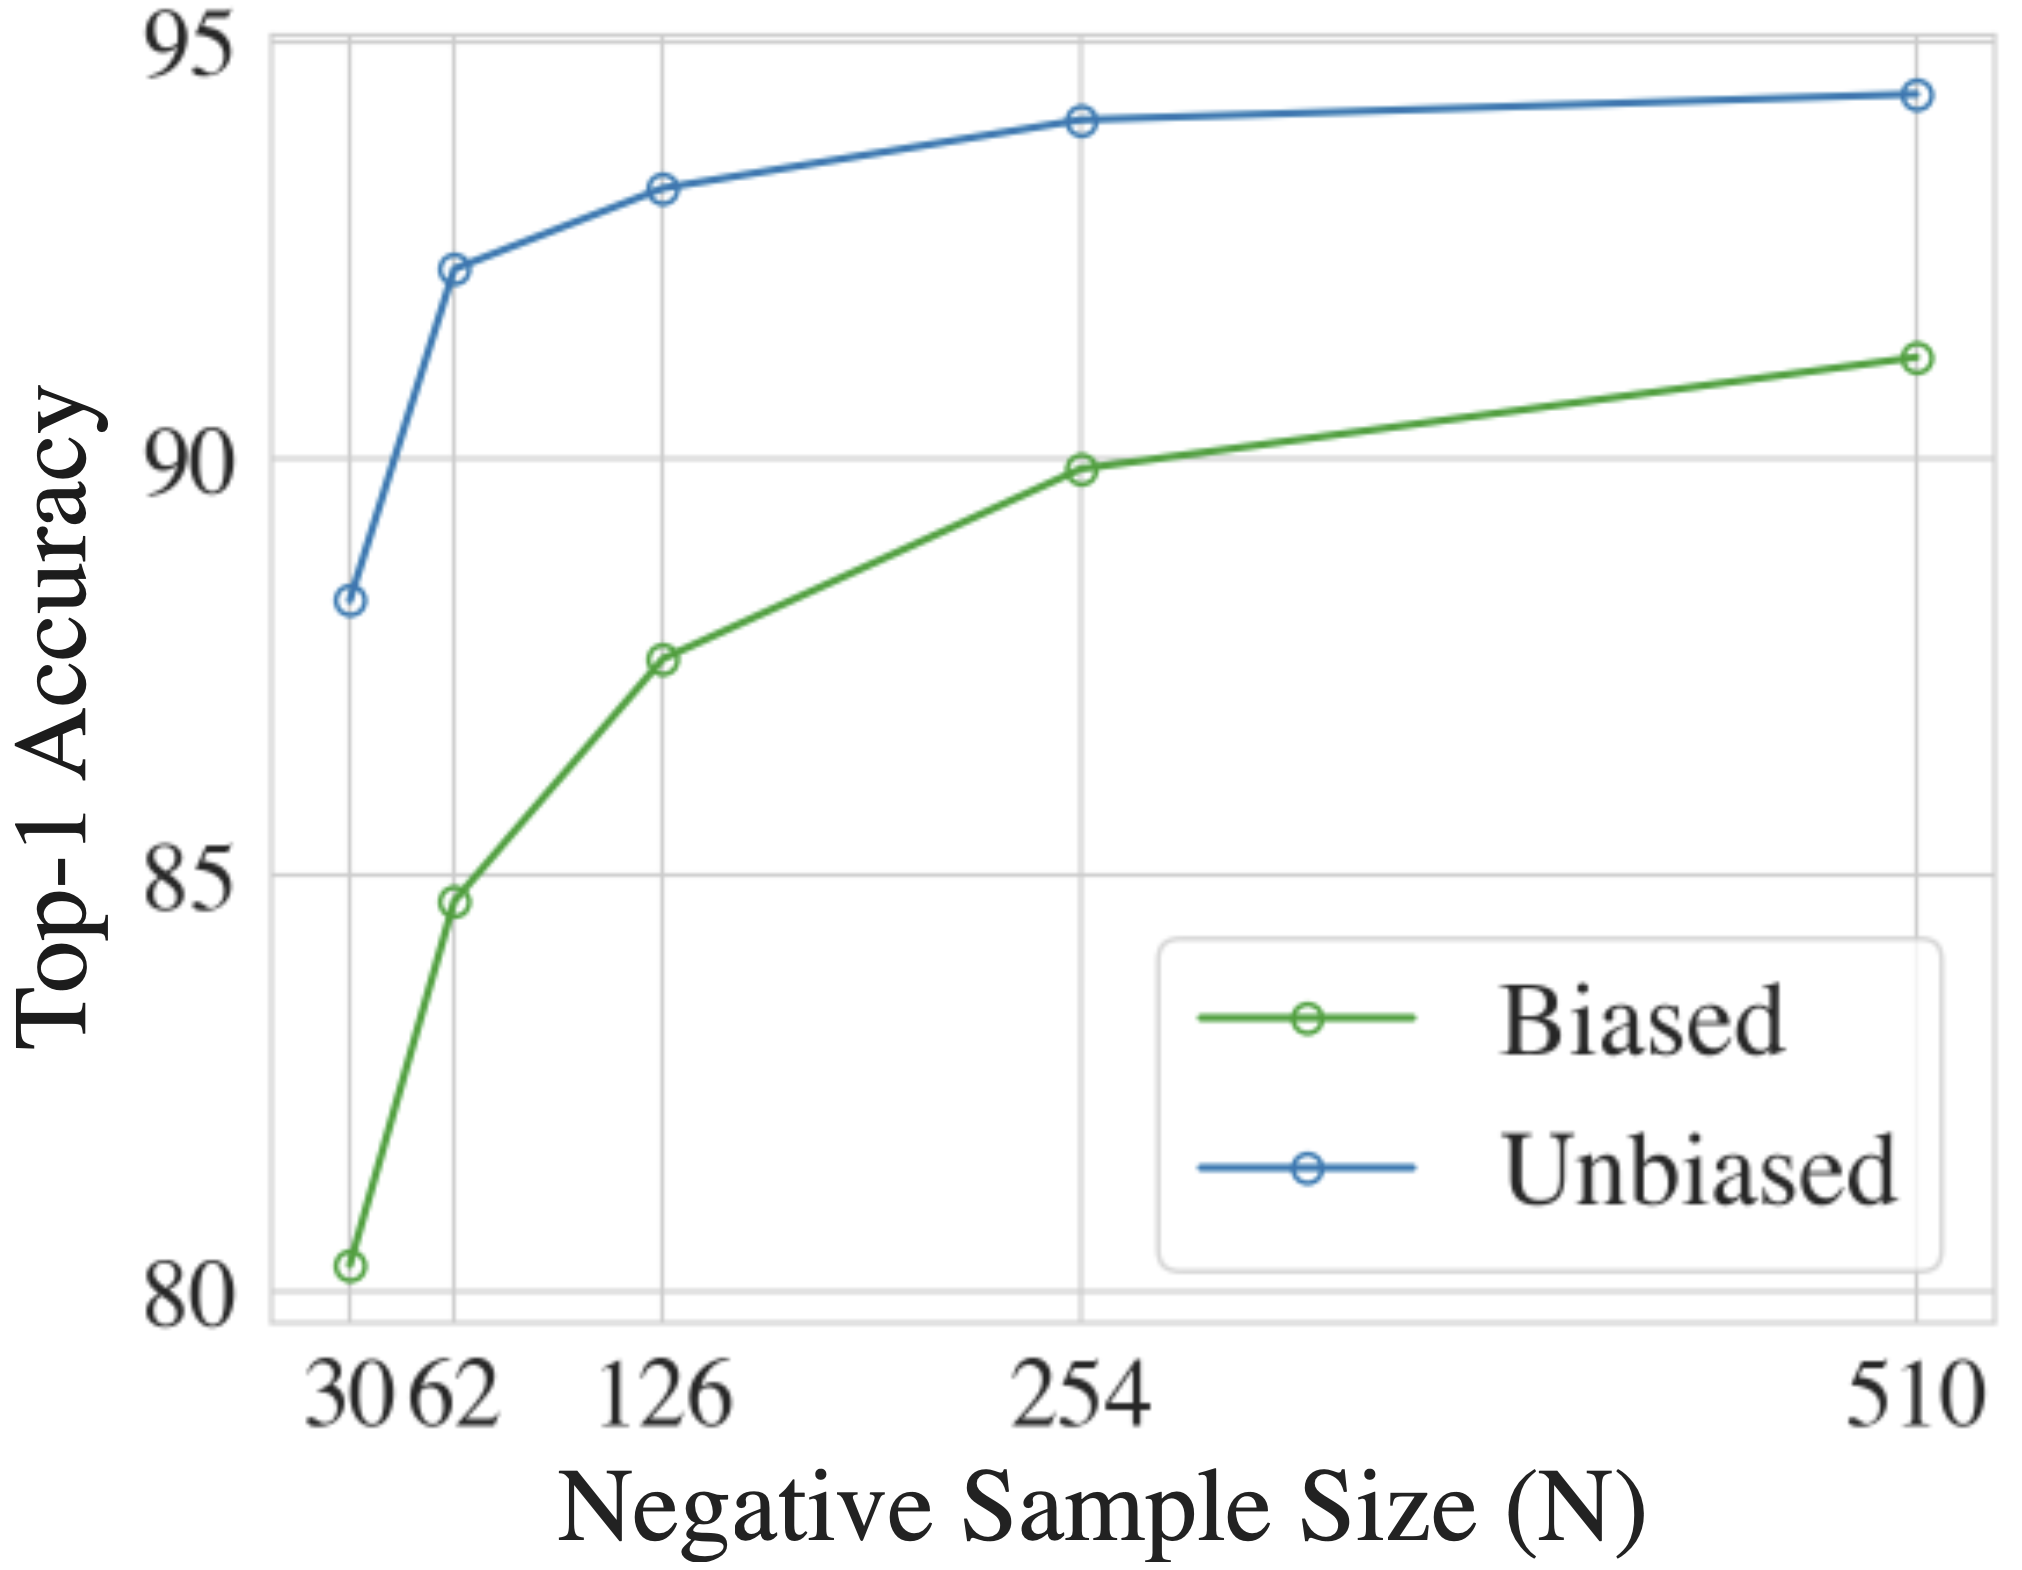
\includegraphics[width=5cm]{images/debiased_sampling_accuracy.png} }}%
    \caption{Visualization of sampling bias and its effect on the model's performance.}%
    \label{fig:sampling_bias}%
\end{figure}

\citeauthor{chuang_debiased_2020} assume a \ac{pu} learning scenario, 
where a positive sample and an unlabeled dataset $p(x)$ are available.
The positive distribution $p^+$ is mimicked by data augmentations.
The empirical estimation of the objective is given in 
\autoref{eq:debiasing_loss} from \citet{chuang_debiased_2020},
which is easier to compute than the original objective.
The negative samples $x^-$ are sampled from the data distribution $p(x)$.
However, the authors added a correction term for positive samples $x^+$.
The weighting factor $Q$ is used to balance the debiasing effect.

\begin{equation}
    \mathbb{E}_{x \sim p; x^+ \sim p^+}[{-\log{\frac{e^{f(x)^Tf(x^+)}}{e^{f(x)^Tf(x^+)}+ \frac{Q}{\tau^-}(\mathbb{E}_{x^- \sim p}[e^{f(x)^Tf(x^-)}]-\tau^+\mathbb{E}_{v \sim p^+}[e^{f(x)^Tf(v)}])}}}]
    \label{eq:debiasing_loss}
\end{equation}


\subsection{\acl{drc}}\label{subsec:drc}

\citeauthor{DRC_2020} propose a method called \ac{drc} 
that faces issues of high intra-class diversities 
due to structural shortcomings in existing deep clustering methods.
They claim that existing methods enforce the representations of samples 
and their augmentations to be assigned to the same cluster,
due to the usage of the maximum sensitivity of the softmax function used during cluster assignment.

\ac{drc} aims to address this issue by considering both the \ac{af} and the \ac{ap} during clustering.
Even though the \ac{ap} can be similar for different samples, their \ac{af} can be different 
as illustrated in \autoref{fig:drc_af_ap}.

\begin{figure}[!htb] % h = here, t = top, b = bottom, p = page of floats
    \centering
    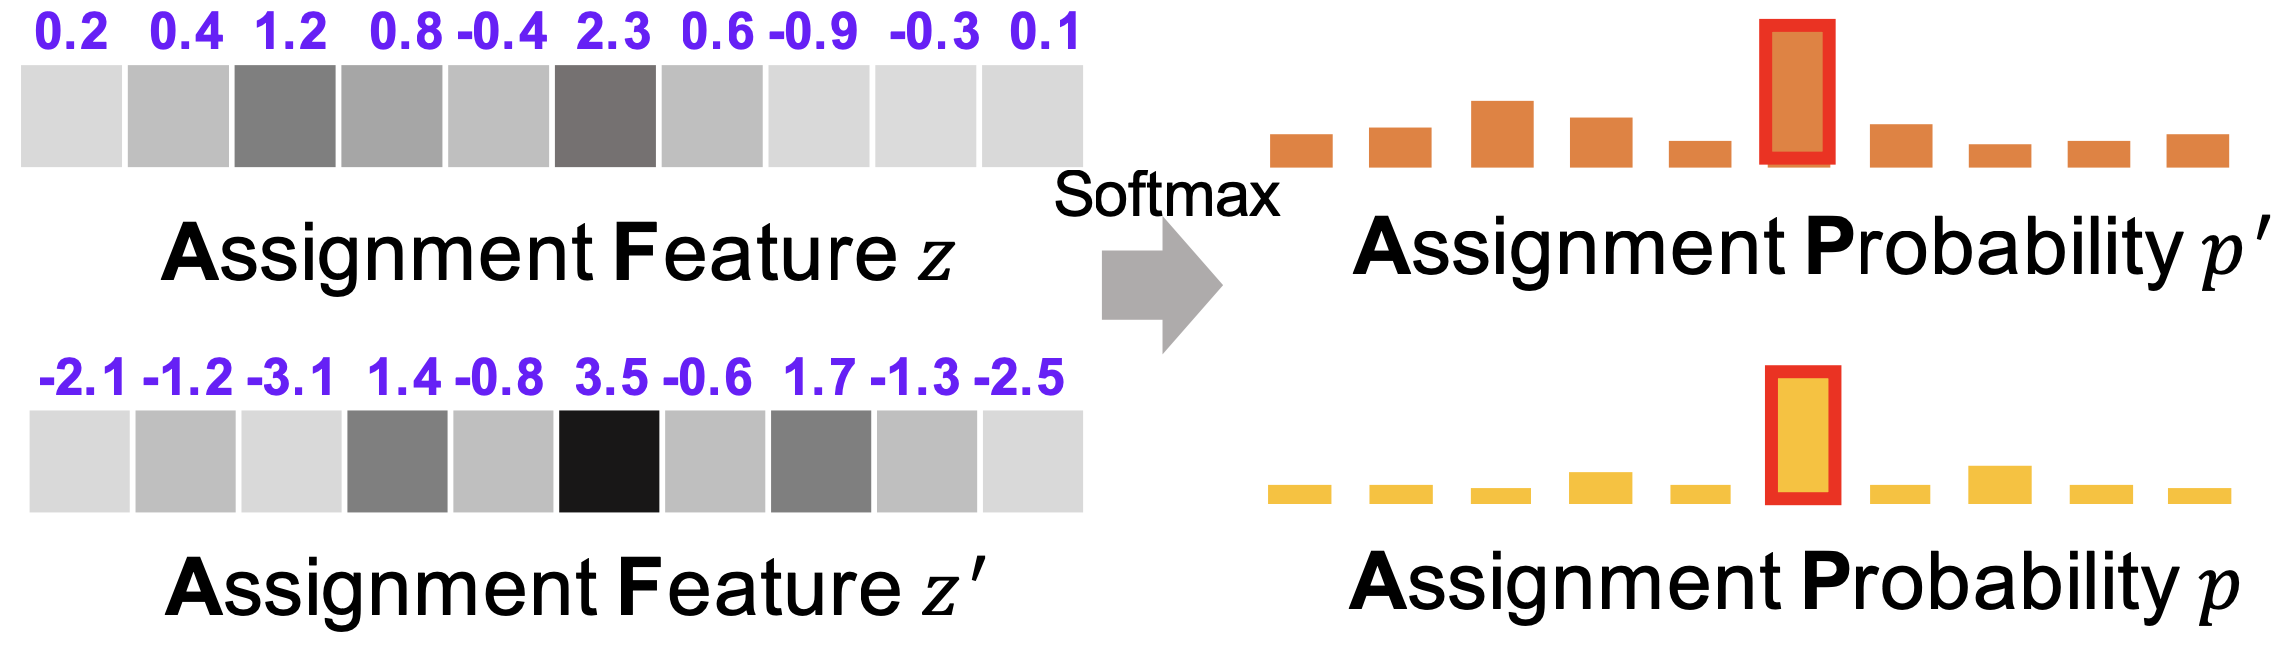
\includegraphics[width=300pt]{images/DRC_af_ap.png}
    \caption{Similar \ac{ap} values for different samples, but different \ac{af} values from \citet{DRC_2020}.
    Cluster assignment based on only \ac{ap} values can result in high intra-cluster diversities.}
    \label{fig:drc_af_ap}
\end{figure}

The \ac{af} $z_i$ are obtained from a \ac{cnn} with a fully connected layer, i.e. $z_i = f_\theta(x_i)$.
The \ac{ap} are obtained from the softmax function from \eqref{eq:ap}. 
Each sample $x_i$ is assigned to the cluster $j$ with the highest \ac{ap} value $p_{ij}$.
Optimally, the samples of a latent class should belong to the same cluster.

\begin{equation}
    p_{ij} = \frac{e^{z_{ij}}}{\sum_{K}^{t=1}e^{z_{it}}}, j \in \left[1,K\right]
    \label{eq:ap}
\end{equation}

\citeauthor{DRC_2020} present the loss function $\mathcal{L} = \mathcal{L}_{AF} + \mathcal{L}_{AP}  + \lambda \mathcal{L}_{CR}$  consisting of three terms.
The first term $\mathcal{L}_{AF}$ is the \ac{af} loss, which enforces similar representations of the sample and its positive transformation.
The second term $\mathcal{L}_{AP}$ is the \ac{ap} loss, which enforces the positive pairs of a sample and its augmentation 
to be assigned to the same cluster.
The third term $\mathcal{L}_{CR}$ is the cluster regularization loss, which penalizes clusterings where most samples are assigned to a minority of clusters.

\subsubsection{\acl{la}}\label{subsec:local_aggregation}

% s. unten: Hyperparameter prob- woher? k, H ist getestet, zumindest das Verhältnis, aber lambda wird aus anderer Arbeit übernommen -> keine Hyperparameter Suche

\citet{local_aggr_2019} optimize a low-dimensional feature space mapping by 
iteratively identifying close neighbours and updating the embedding function.
This soft clustering technique is called \ac{la}.

At each step during training of the embedding function $f_\theta: \mathcal{X} \rightarrow \mathcal{Z}$, 
two sets of neighbours are identified for each datapoint's embedding $z_i$ 
which are illustrated in \autoref{fig:la_bi_ci}.
The first set $C_i$ contains $z_i$'s close neighbours in the feature space, while
the second set $B_i$ contains $z_i$'s background neighbours.
$B_i$ is used as a means to judge distance and similarity, 
while $C_i$'s members should be embedded closer to $z_i$.
In other words, $C_i$ can be considered the set of positive samples while 
$B_i$ denotes the set of negative samples.
The level of \ac{la} $L(C_i,B_i | \theta, x_i)$ 
characterizes the relative level of closeness within $C_i$ compared to $B_i$.
$L(C_i,B_i | \theta, x_i)$ should be maximized.

The set $B_i$ consists of the $k$ nearest neighbours of $z_i$ in terms of cosine distance 
in the feature space.
$k$ is a hyperparameter and \citet{local_aggr_2019} set $k=4096$.
In order to construct $C_i$, 
first $H$ $k$-means clusterings are performed with sligthly different conditions.
Then, all of $z_i$'s clusters are united to form $C_i$.
$H$ and $k$ are hyperparameters.
\citet{local_aggr_2019} find that more clusterings, i.e. higher $H$, lead to isotropic clusters since outliers which arise from random processes are averaged out.
If $H$ is too high compared to the number of clusters $k$, the performance decreases.
They state that $H=3, k=10000$ and $H=10, k=30000$ are better values than $H=10, k=10000$ 
in terms of ResNet-18 nearest neighbour validation performance.

Finally, the level of \ac{la} $L(C_i,B_i | \theta, x_i)$ is defined as the negative log-likelihood 
of the feature space representation $z_i$ of $x_i$ being in $C_i$ given $B_i$, 
i.e., being recognized as a close neighbour given being recognized as a background neighbour.
The loss to minimize is $\mathcal{L} = L(C_i,B_i | \theta, x_i) + \lambda \left\| \theta \right\|^2$.
\citet{local_aggr_2019} choose to rely on hyperparameter settings from another work rather than conducting a hyperparameter search.

\begin{figure}[!htb] % h = here, t = top, b = bottom, p = page of floats
    \centering
    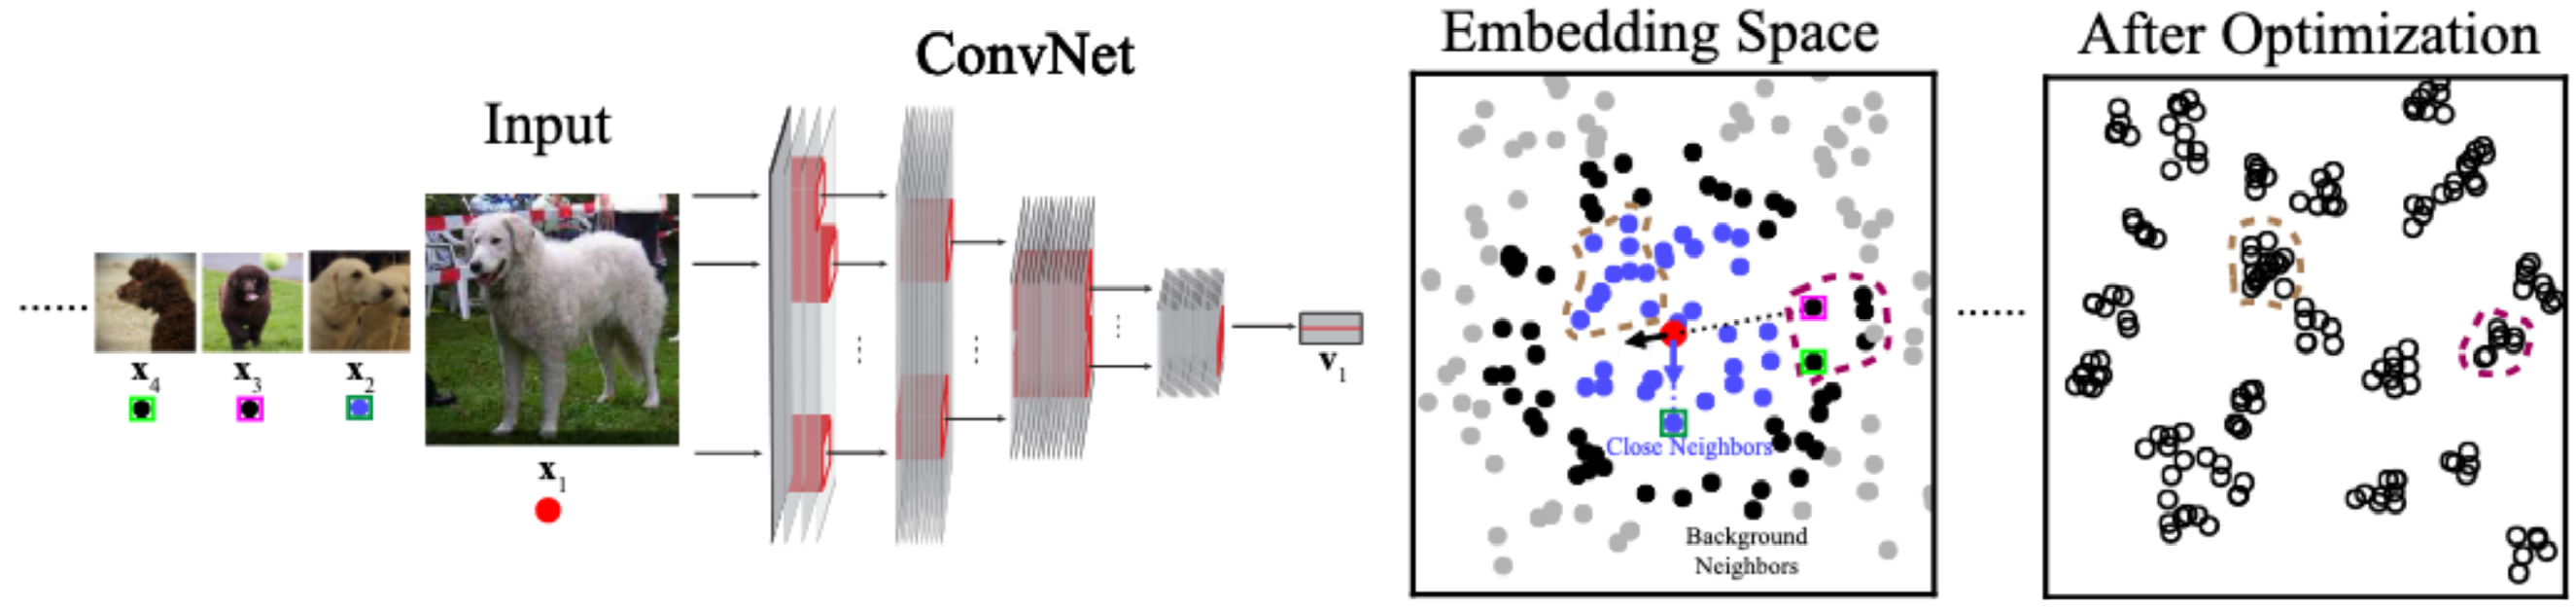
\includegraphics[width=360pt]{images/la_neighbourhoods.png}
    \caption{Illustration from \citet{local_aggr_2019}.
    A \ac{cnn} produces the feature space embedding $z_i = f_\theta(x_i)$.
    The embeddings are displayed as points in the feature space.
    The red point is the anchor $z_i$, 
    whereas blue points are close neighbours $C_i$ and
    black points are background neighbours $B_i$.
    The arrows denote influences between the neighbours.}
    \label{fig:la_bi_ci}
\end{figure}

\subsubsection{Mining on manifolds}\label{subsec:mining_manifolds}


% sparse usage of hard pairs inspired by SVMs

% purpose
According to \citet{mining_manifolds_2018}, the initial representation of the data is obtained by e.g. a pre-trained \ac{cnn}.
Hard pair mining is performed in order to fine-tune the network.

% idea of positive and negative samples
For fine-tuning, a combination of different definitions of proximity induces mining 
for hard positives and negatives as displayed in \autoref{fig:mining_manifolds_vis}.
Given an anchor, samples that reside on the same manifold but 
are not proximate in terms of Euclidean distance are considered hard positive samples.
These positive samples should be embedded closer to the anchor in the Euclidean space.
Conversely, hard negative samples are those that are spatially proximate in Euclidean space 
yet lie on different manifolds.
These samples should be embedded further away from the anchor in the Euclidean space.
%The hard samples are mined from an unordered set of \textit{relevant} samples.

% different neighbourhoods & hard samples
The authors denote the set of the $k$ nearest Euclidean neighbours $NN^e_k$ and 
the $k$ nearest manifold neighbours $NN^m_k$.
The hard positives are defined as $NN^m_k \textbackslash NN^e_k$. 
The pool $NN^m_k$ is ordered by descending manifold similarity to the anchor
to ensure that high-confidence samples are chosen first.
$k$ controls the diversity of the hard positives.
The larger $k$ is, the more diverse, i.e. hard, the hard positives are. 
The pool of hard negatives is defined as $NN^e_k \textbackslash NN^m_k$.
$NN^e_k$ is ordered by descending Euclidean distance to the anchor to keep the hardest samples.

% visualization of hard samples
\begin{figure}[!htb]% h = here, t = top, b = bottom, p = page of floats
    \centering
    \subfloat[\centering $k$ nearest Euclidean neighbour $NN^e_k$ (orange).]
    {{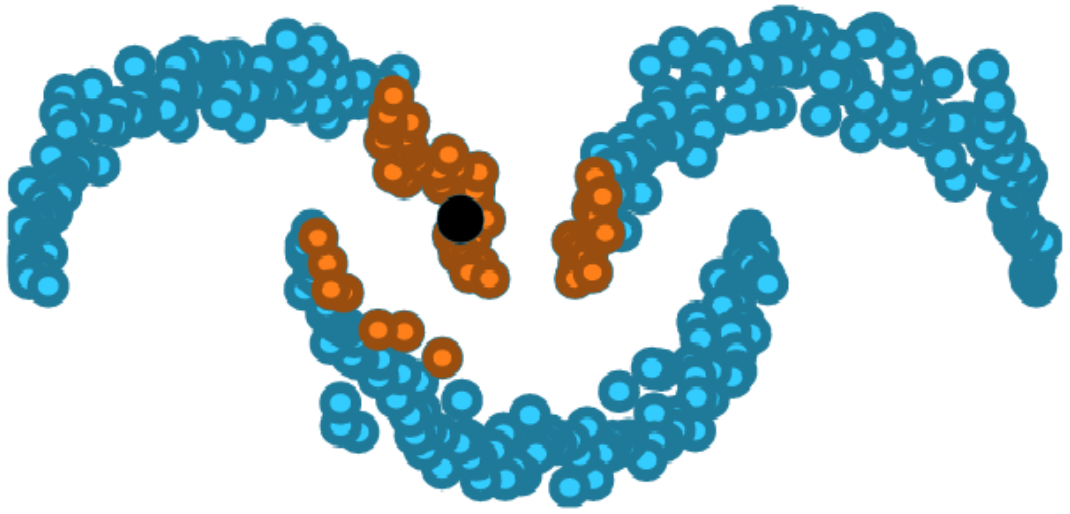
\includegraphics[width=5cm]{images/euclidean_NN.png} }}%
    \qquad
    \subfloat[\centering $k$ nearest manifold neighbour $NN^m_k$ (purple).]
    {{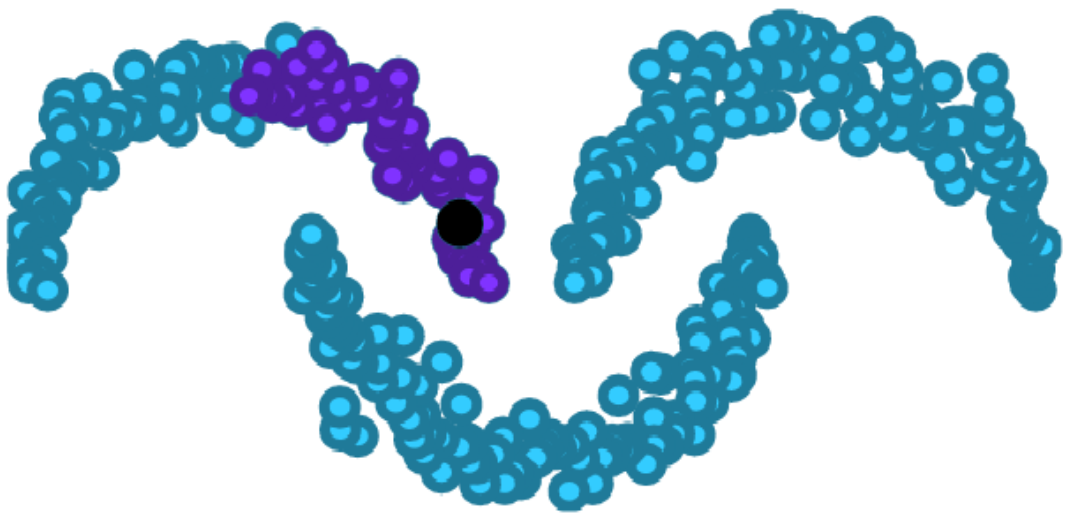
\includegraphics[width=5cm]{images/manifold_NN.png} }}%
    \qquad
    \subfloat[\centering Hard positives $NN^m_k \textbackslash NN^e_k$(green).]
    {{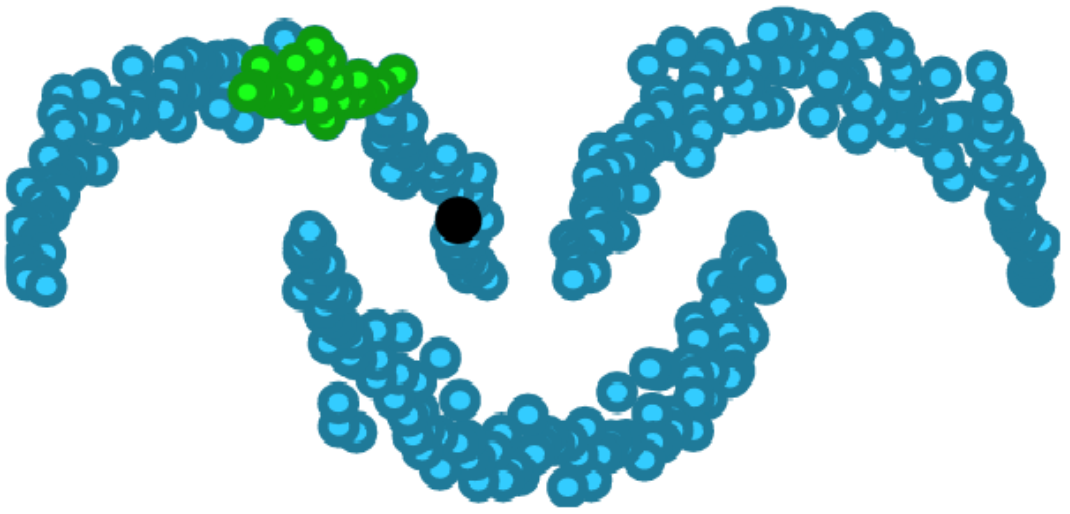
\includegraphics[width=5cm]{images/hard_positives_manifold.png} }}%
    \qquad
    \subfloat[\centering Hard negatives $NN^e_k \textbackslash NN^m_k$(red).]
    {{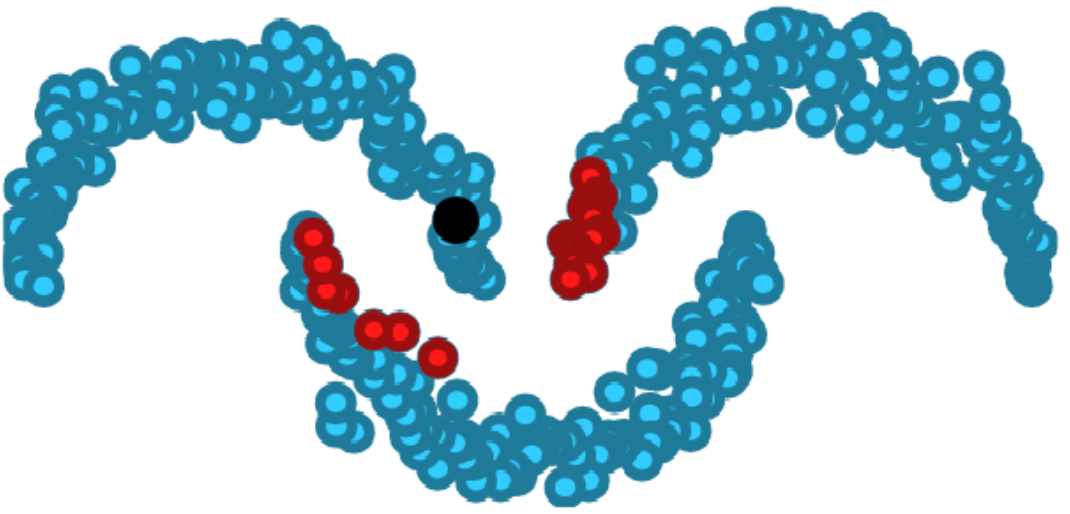
\includegraphics[width=5cm]{images/hard_negatives_euclidean.png} }}%

    \caption{Visualization of different proximity definitions, 
    the hard negatives and positives from \citet{mining_manifolds_2018}.
    The anchor is the black point.}%
    \label{fig:mining_manifolds_vis}%
\end{figure}


% manifolds via random walk n nearest neighbour graph
\citet{mining_manifolds_2018} propose a method where the manifold is estimated by mode-seeking, i.e. a random walk process, 
on the Euclidean nearest neighbour graph induced by the Euclidean similarity function $s_e$.
The graph is undirected, weighted and represented by a sparse symmetric adjacency matrix.
The adjacency matrix is constructed from the reciprocal $k$ nearest neighbours of each sample, 
where two points are considered reciprocal if each belongs to the $k$ nearest neighbours of the other. 
To reduce the negative impact of outliers, only reciprocal nearest neighbours are incorporated \citep{diffusion_2017,mining_manifolds_2018,fast_2018}.
The weighted adjacency matrix entries $a_{ij}$ defined in \Eqref{eq:mining_manifolds_adjacency_matrix} from \citet{mining_manifolds_2018} 
are calculated via the Euclidean distance between the samples if both nodes are in each other's nearest neighbourhood.
Diagonal entries are set to zero \citep{mining_manifolds_2018,fast_2018}.
%They admit that assessing the manifold similarity poses additional computational and memory requirements.
The manifold is computed once at the beginning \citep{mining_manifolds_2018}.

\begin{equation}
    a_{ij} = \begin{cases}
        s_e(y_i,y_j), & \text{if } y_i \in NN^e_k(y_j)\wedge y_j \in NN^e_k(y_i)\\
        0, & \text{otherwise}\\
      \end{cases}     
    \label{eq:mining_manifolds_adjacency_matrix}
\end{equation}


% mode seeking
% The manifold representation is obtained via mode-seeking as described in \citet{mode_seeking_2012}.
% The nearest neighbour network consists of samples as nodes and is weighted by the Euclidean distance 
% if both samples are in each other's $k$ nearest neighbourhood \citet{mode_seeking_2012,mining_manifolds_2018}.

% authority modes
While traditional mode-seeking relies on metric features, such as distances, mode-seeking on graphs 
uses the concept of random walks instead \citep{mode_seeking_2012}.
A random walk, i.e. a linear combination of the identity matrix and a scaled version of the adjacency matrix, is simulated multiple times on the graph.
\citet{mode_seeking_2012} define the so-called authority modes on a graph 
as the most frequently visited nodes by random walks among their local neighbours.
They correspond to the local maxima of the underlying probability distribution of random walks over the graph.
% selection of anchors
Since the anchors should be diverse and relevant, they are chosen to be the authority modes \citep{mining_manifolds_2018}.

% authority score
Inspired by PageRank, the possibility of random jumps is included in order to ensure convergence to a stationary distribution. 
The probability of visiting a node is denoted by the authority score $\pi$ 
which is defined in \Eqref{eq:authority_score} from \citet{mode_seeking_2012} 
where $p(i,j)$ are the entries of the Markov transition matrix $P$.
$\pi(j)$ takes into account the probability of visiting a node $j$ from a node $i$ and 
the probability of a random jump from one of the nodes chosen uniformly at random.
\citet{mode_seeking_2012} set $\alpha$ to $0.9$. 
The authority score $\pi$ can be computed by, for instance, the power method \citep{mode_seeking_2012,PageRank_2004}.

\begin{equation}
    \pi(j) = \alpha \sum_{i \in \mathcal{V}}^{}  \pi(i)p(i,j) + (1-\alpha)\frac{1}{N} , \text{ where } p(i,j) = \frac{a_{ij} }{\sum_{k \in \mathcal{V}}^{}a_{ik} } 
    \label{eq:authority_score}
\end{equation}

% local neighbours on the manifold: node relevancy 
\citet{mode_seeking_2012} define node relevancy $\Psi(s,t)$ via \Eqref{eq:node_relevancy} where $d(s)$ denotes the out-degree of a node.
To incorporate the reachability of a node, the probability of reaching node $t$ from node $s$ in $k$ steps $p_k(s,t)$ is 
defined via the $k_{th}$ power of the Markov transition matrix $P$.
To support similar authority scores between neighbouring nodes, the exponential term including a weighting factor $\gamma$ is included.
$\Psi(s,t)$ is not symmetric and depends on the random walk step $k$.
The authors propose to use the node relevancy $\Psi(s,t)$ for a node $s$ to determine the manifold neighbours $N_\varepsilon^m(s)$ for $s$ 
via the usage of a threshold $\varepsilon$: 
$N_\varepsilon^m(s) =  \left\{ t \in \mathcal{V} | \Psi(s,t) > \varepsilon \right\} \cup \left\{ s \right\}$ \citep{mode_seeking_2012}.

\begin{equation}
    \Psi(s,t) = d(s) p_k(s,t) \exp(-\gamma \left\{  \pi(t) - \pi(s)  \right\}^2)\text{, where } d(s) = \sum_{j\in \mathcal{V}}^{}a_{sj}
    \label{eq:node_relevancy}
\end{equation}

% AAS
They propose the \ac{aas} as a nonparametric estimator of the authority modes.
A node $s$ is shifted to node $\mathcal{A}(s)$ calculated in \Eqref{eq:authority_ascent_shift}. 
This formula chooses the local neighbour $t$ of $s$ that maximizes the difference of the authority scores $\pi$.
The authors argue that the \ac{aas} is finite and converges since the graph is finite.
When \ac{aas} is completed, manifolds are represented as clusters.
% examples
Resulting hard positives and negatives are displayed in \autoref{fig:manifold_mining_qualitative_analysis} and \autoref{fig:manifold_mining_examples}.

\begin{equation}
    \mathcal{A}(s) = \underset{t \in \mathcal{N_\varepsilon}(s)}{\text{argmax}} \left\{ p_k(s,t)\left[ \pi(t)-\pi(s) \right] \right\}
    \label{eq:authority_ascent_shift}
\end{equation}

% inlier and outlier
% Inliers on the manifold reside in large clusters while outliers are isolated in small groups since they do not have enough relevancy with inliers \citet{mode_seeking_2012}.
% Hence, outlier clusters can be identified by low sums of authority values.


\begin{figure}[!htb] % h = here, t = top, b = bottom, p = page of floats
    \centering
    \includegraphics[width=300pt]{images/mining_manifold_qualitative_analysis.png}
    \caption{Illustration of CUB200-2011 from \citet{mining_manifolds_2018}.
    The anchor is denoted $x^r$.
    A selection of hard positives from $P^+(x^r)$ is compared to the 
    baseline approach that samples from the closest neighbours to $x^r$ in 
    terms of Euclidean distance.
    Analogously, a selection of hard negatives from $P^-(x^r)$ 
    is compared to the baseline $X \textbackslash NN^e_3$, 
    i.e. sampling from the set that contains all samples but the three closest ones in 
    terms of Euclidean distance.
    The borders of the images denote the ground-truth class, i.e. if bird species is the same.
    Green borders indicate that the image belongs to the same class as the anchor, 
    while red borders signify images from a different class.
    It becomes apparent that the sampled hard positives consist of fewer false positives 
    than the baseline.
    }
    \label{fig:manifold_mining_qualitative_analysis}
\end{figure}

\begin{figure}[!htb] % h = here, t = top, b = bottom, p = page of floats
    \centering
    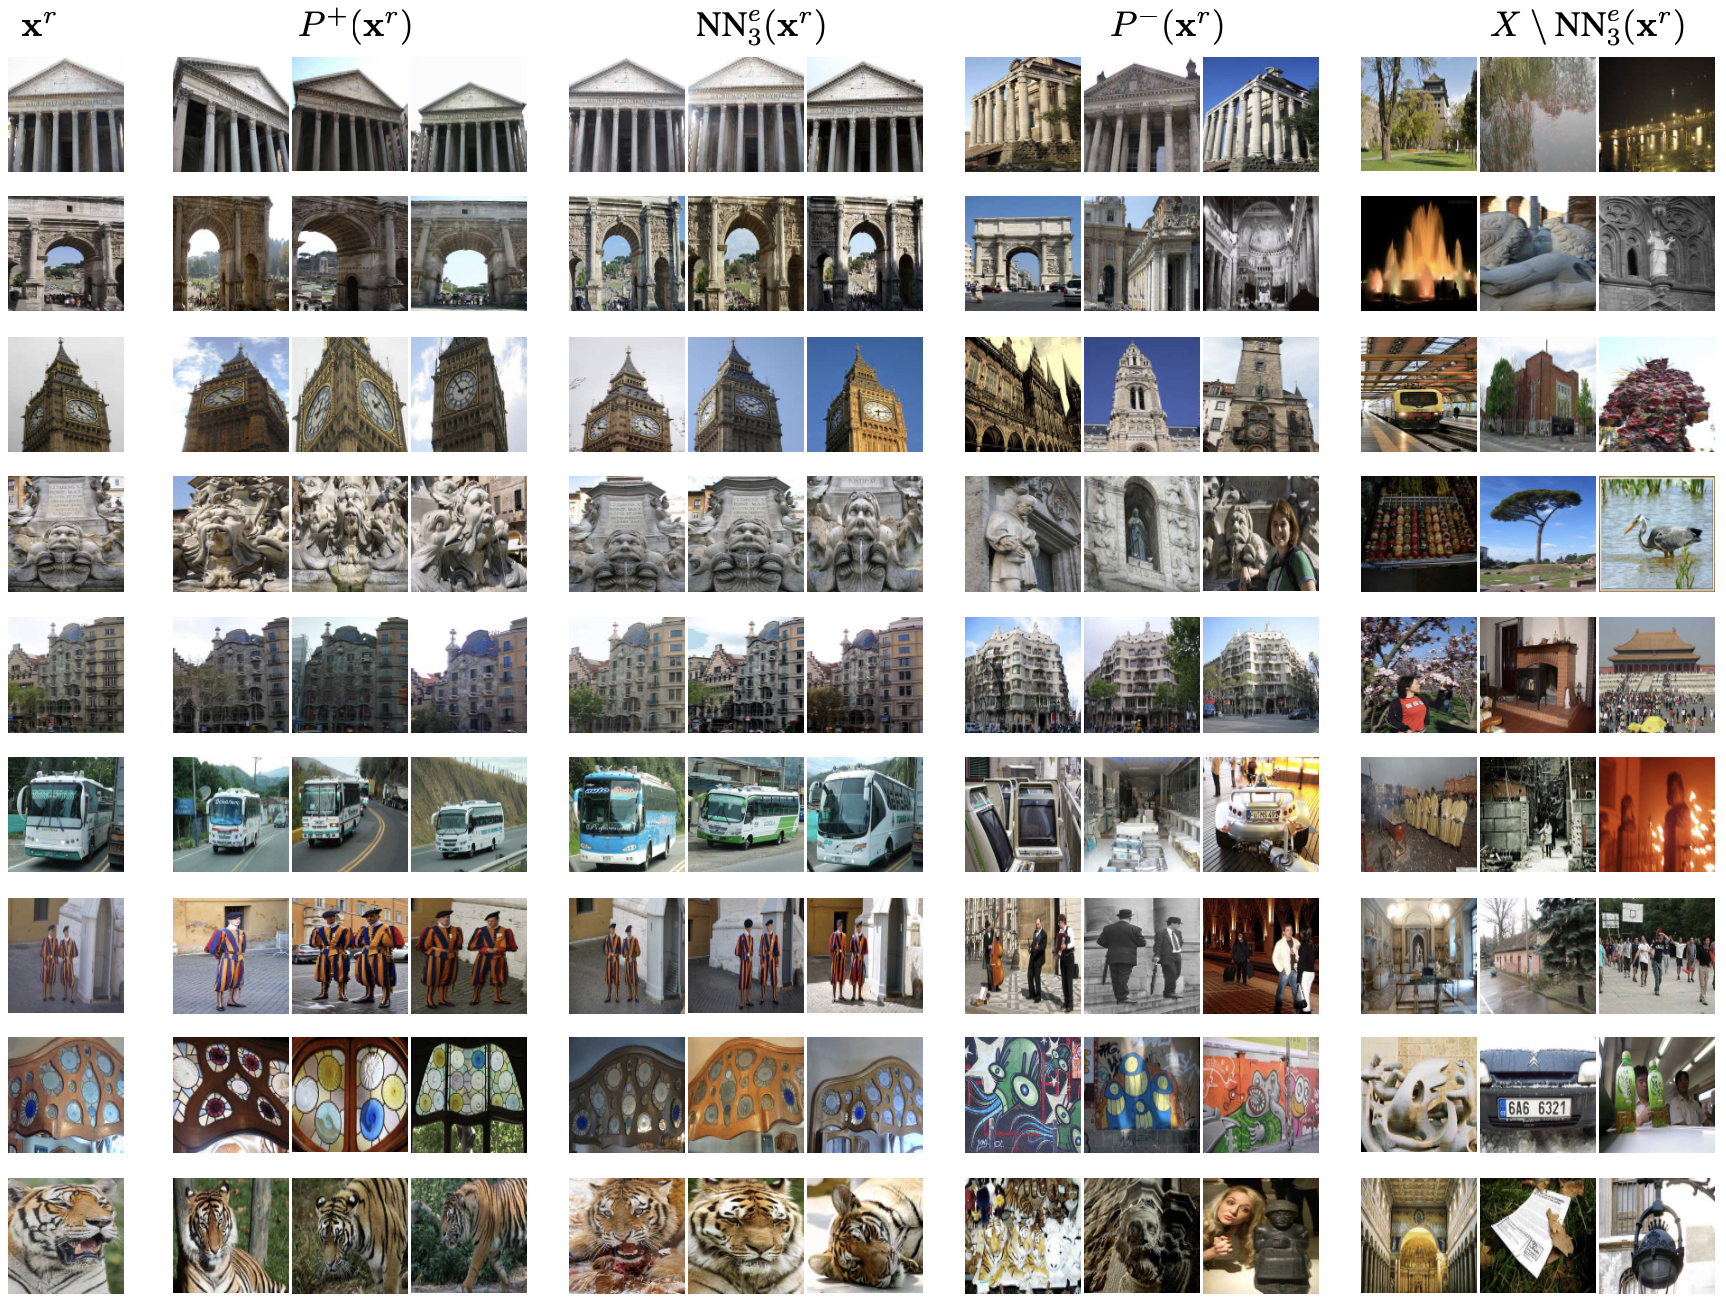
\includegraphics[width=360pt]{images/mining_manifold_examples.png}
    \caption{Illustration Oxford5k and Paris6k images crawled from Flickr from \citet{mining_manifolds_2018}.
    The dataset contains multiple images for each landmark building, i.e. class \citep{manifold_dataset}.
    The anchor is denoted $x^r$.
    A selection of hard positives from $P^+(x^r)$ is compared to the 
    baseline approach that samples from the closest neighbours to $x^r$ in 
    terms of Euclidean distance.
    Analogously, a selection of hard negatives from $P^-(x^r)$ 
    is compared to the baseline $X \textbackslash NN^e_3$, 
    i.e. sampling from the set that contains all samples but the three closest ones in 
    terms of Euclidean distance.
    It becomes apparent that the hard negatives display visually similar but 
    semantically different images to the anchor. % good
    }
    \label{fig:manifold_mining_examples}
\end{figure}

% loss functions
The authors propose multiple loss functions to train the model.
They, for instance, apply the contrastive loss $l_c(x^r, x^+, x^-)= \left\| x^r - x^+ \right\|^2 + \left[ m - \left\| x^r - x^- \right\| \right]^2$, 
the triplet loss $l_t(x^r, x^+, x^-)= \left[ m +  \left\| x^r - x^+ \right\| ^2 - \left\| x^r - x^- \right\| \right]^2$, 
and weighted versions of both contrastive and triplet loss, where the loss is multiplied by the manifold similarity of anchor and positive sample \citep{mining_manifolds_2018}.
$m$ is a margin parameter and $x^r$ is the representation of the anchor.

\subsection{\acl{mochi}}\label{subsec:MoCHi}

\citet{mochi_2020} claim that most approaches to sampling negatives rely on 
time-consuming updates of a memory bank or big batches to achieve good performance.
They propose \ac{mochi}, a method that computes samples online claiming without any computational overhead.

% memory bank
They use a memory bank $Q$ of size $| Q | = K$ to store negative samples.
There are different ways to choose $K$ by either saving the whole dataset, a queue of the last batches,
or all images in the current batch.

% definition of MoCHi
The definition of \ac{mochi}($N, s, s'$) is as follows:
\begin{enumerate}
    \item $N$: Number of negative samples from the memory bank to consider during negative mining.
    \item $s$: Number of samples to generate with approach 1.
    \item $s'$: Number of samples to generate with approach 2.
\end{enumerate}
For both approaches to generating negative samples, the authors use the same memory bank $Q$.
Given a fixed anchor, firstly, $Q$ is ordered in descending similarity to the anchor representation    
in the feature space producing $\tilde{Q}$.
The similarity between $n_j \in \tilde{Q}$ and the query $q$ is calculated via 
a scaled dot product of both samples.
Secondly, all but the first, i.e. most similar, $N$ samples are discarded from $\tilde{Q}$.
% first approach
The first approach proposed by \citeauthor{mochi_2020}, chooses two random samples $n_i, n_j \in \tilde{Q}$ 
and a mixing coefficient $\alpha_k \in (0,1)$, 
to generate the new sample as a linear combination of the existing hard negative samples 
as described in \eqref{eq:mochi_appr1}.

\begin{equation}
    h_k = \frac{\tilde{h_k}}{\left\| \tilde{h_k}  \right\|}; \tilde{h_k} = \alpha_k n_i + (1-\alpha_k)n_j
    \label{eq:mochi_appr1}
\end{equation}

% second approach
The second approach generates new samples by using the anchor representation $q$ 
and a random sample $n_j \in \tilde{Q}$ to generate the new sample as described in \eqref{eq:mochi_appr2}.
The mixing coefficient $\beta_k \in (0,0.5)$ is used to balance the influence of the anchor 
and the hard negative sample.
By limiting the influence of the anchor, the authors enforce a stronger influence of the negative sample.
This approach is considered to produce even harder negative samples than the first approach.

\begin{equation}
    h_k' = \frac{\tilde{h_k'}}{\left\| \tilde{h_k'}  \right\|}; \tilde{h_k'} = \beta q + (1-\beta_k)n_j
    \label{eq:mochi_appr2}
\end{equation}

% update of memory bank
Using \eqref{eq:mochi_appr1} and \eqref{eq:mochi_appr2}, 
$s$ and $s'$ hard negative samples are generated respectively.
Afterward, the similarity of each generated sample $h_k$ (or $h_k'$ respectively) 
to the anchor $q$ is calculated via $\frac{q^T h_k}{\tau}$.
This similarity is used to update the memory bank $\tilde{Q}$ 
by inserting the new sample.

% loss functions
There are two loss functions proposed by \citet{mochi_2020} to train the model.
Firstly, the alignment loss is used to determine 
the absolute distance between representations with the same class label.
Secondly, the uniformity loss is used to determine 
the distribution of representations on the hyperphere.
It is calculated via the logarithm of the average pairwise Gaussian potential between all embeddings.

% s, s' effect
\citet{mochi_2020} conducted experiments to investigate the effect of the parameters $s, s'$.
They present metrics such as average precision and accuracy for different ratios of $s$ and $s'$ 
for object detection and image segmentation tasks on COCO as well as 
linear classification on ImageNet-1K and object detection on PASCAL VOC.
Generally, the scores differ only in magnitudes of $1 \%$.
Additionally, the authors state that for $s > 0, s' = 0$ the model learns faster but achieves similar performance to the baseline, i.e. the model without \ac{mochi}.


% modifications
The authors listed modifications to \ac{mochi} that lead to inferior performance.
They tried to define the mixing coefficient via the similarity of the hard negative samples 
to the anchor. % how negative the sample is 
Moreover, they introduced non-uniformity when sampling $n_i, n_j$ from $\tilde{Q}$ by defining a 
probability distribution over similarities to the query. % too hard samples
Alternatively, they proposed omitting the parameters $s, s'$ and 
sampling hard negatives using alternately approaches 1 and 2 until $N\%$ of the top samples in 
$\tilde{Q}$ correspond to synthesized samples.

% scheme 2 from ProGCL: ProGCL-mix (MoCHi)
\begin{equation}
    \tilde{h_k} =  \alpha_k \cdot n_i + (1-\alpha_k) \cdot  n_j, \text{ where } \alpha_k = \frac{p(n_i \text{ is } TP)}{p(n_i \text{ is } TP) + p(n_j \text{ is } TP)}
    \label{eq:progcl_mix}
\end{equation}

The researches that introduced \progcl{} (\autoref{subsec:graph_distribution}) in \citet{progcl_2022} 
present an extension of the hard mining strategy \ac{mochi}.% introduced in \autoref{subsec:MoCHi}.
They claim, that a high portion of the negative samples generated by \ac{mochi} are \acp{fn}.
They therefore propose to weigh the selected negative samples for mixing 
according to their relative probability of being a \ac{tn} as displayed in \eqref{eq:progcl_mix}.

\subsubsection{\acl{pcl}}\label{subsec:PCL}

\citet{PCL_2021} use clustering in the feature space to optimize the sample's representation.
Each sample is associated with $M$ prototypes, which are obtained through $k_m$-means clustering across various values of $m$.
These prototypes, represented by cluster centroids, act as latent variables and are classified as positive samples. 
A contrastive loss is applied to ensure that the sample's embedding aligns closely with its assigned prototypes.
The so-called prototypical contrastive loss ProtoNCE is optimized using an \ac{em} algorithm 
as displayed in \autoref{fig:PCL_training}.

\begin{figure}[!htb] % h = here, t = top, b = bottom, p = page of floats
    \centering
    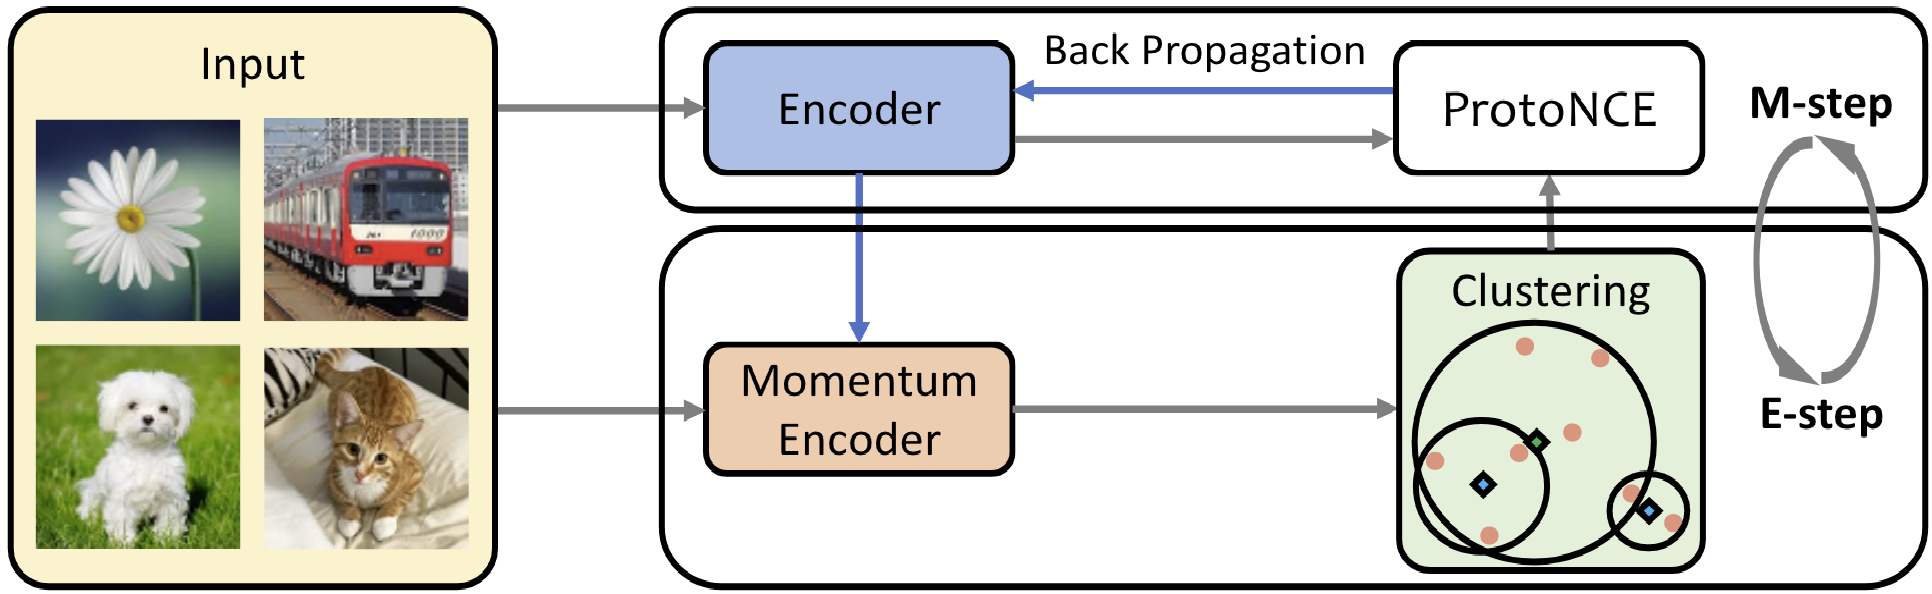
\includegraphics[width=360pt]{images/PCL_training.png}
    \caption{Illustration from \citet{PCL_2021}.
    The training process of the \ac{pcl} algorithm is demonstrated.
    $M$ $k_m$-means clusterings based on the feature space defined by the momentum encoder 
    are performed in the E-step.
    The prototypes $c^m_{\tilde{k}}$, $\tilde{k} \in [1, k_m]$, illustrated as green/ blue rectangles, 
    are the cluster centroids.
    The M-step updates the network parameters $\theta$ by optimizing the ProtoNCE loss.
    }
    \label{fig:PCL_training}
\end{figure}

% E-step: define k clusters & momentum encoder
$k$-means clustering is used to find the prototypes in the E-step.
The clustering is performed on the samples' embeddings obtained from the momentum encoder, 
whose parameters are a moving average of the main encoder's parameters and thus, smoother \citep{PCL_2021}.

% M-step
The M-step updates the network parameters $\theta$ by optimizing the ProtoNCE loss.
The minimization of the ProtoNCE loss is equivalent to maximizing the estimated log-likelihood.
The optimal parameters are those that map a sample close to its prototypes.
The result is obtained under the assumptions of a uniform prior over the cluster centroids, i.e. prototypes,
and an isotropic Gaussian distribution of the sample's embeddings around the prototypes.

% ProtoNCE loss
The ProtoNCE loss from \Eqref{eq:ProtoNCE} extends the InfoNCE from \Eqref{eq:InfoNCE} 
by not only enforcing similarity between the sample $z_i$ and 
one positive sample $z_i'$ while retaining dissimilarity to $r$ negative samples $z_j'$, 
but also considering its prototypes $c^m_s$. 
To enhance the stability of the results, $M$ clusterings are performed with varying numbers of clusters $k_m$. 
The use of different $k_m$ introduces varying levels of granularity among the prototypes, 
thereby encoding a hierarchical structure into the loss function.

\begin{equation}
    \mathcal{L}_{InfoNCE}= - \sum_{i=1}^{N}\log\frac{\exp \frac{z_i\cdot z_i'}{\tau}}{\sum_{j=0}^{r}\exp \frac{z_i\cdot z_j'}{\tau}}
    \label{eq:InfoNCE}
\end{equation}

\begin{equation}
    \mathcal{L}_{ProtoNCE}=\mathcal{L}_{InfoNCE} - \sum_{i=1}^{N} \frac{1}{M} \sum_{m=1}^{M} \log\frac{\exp \frac{z_i\cdot c_s^m}{\phi^m_s}}{\sum_{j=0}^{k_m}\exp \frac{z_i\cdot c_j^m}{\phi^m_j}}
    \label{eq:ProtoNCE}
\end{equation}




\subsection{\acl{pic}}\label{subsec:PIC}

\citet{PIC_2020} critize that dual branch, i.e. negative and positive sample sets, 
and epoch-based sampling strategies suffer from information leakage and 
the fact that individual instances are not visited frequently enough.
\ac{pic} is a one-branch method, i.e. only one random augmentation is applied to the input per iteration.
Moreover, \ac{pic} uses a sliding window based data scheduler 
as illustrated in \autoref{fig:pic_data_scheduler}
to ensure that the majority of instances are visited frequently.

\begin{figure}[h] % h = here, t = top, b = bottom, p = page of floats
    \centering
    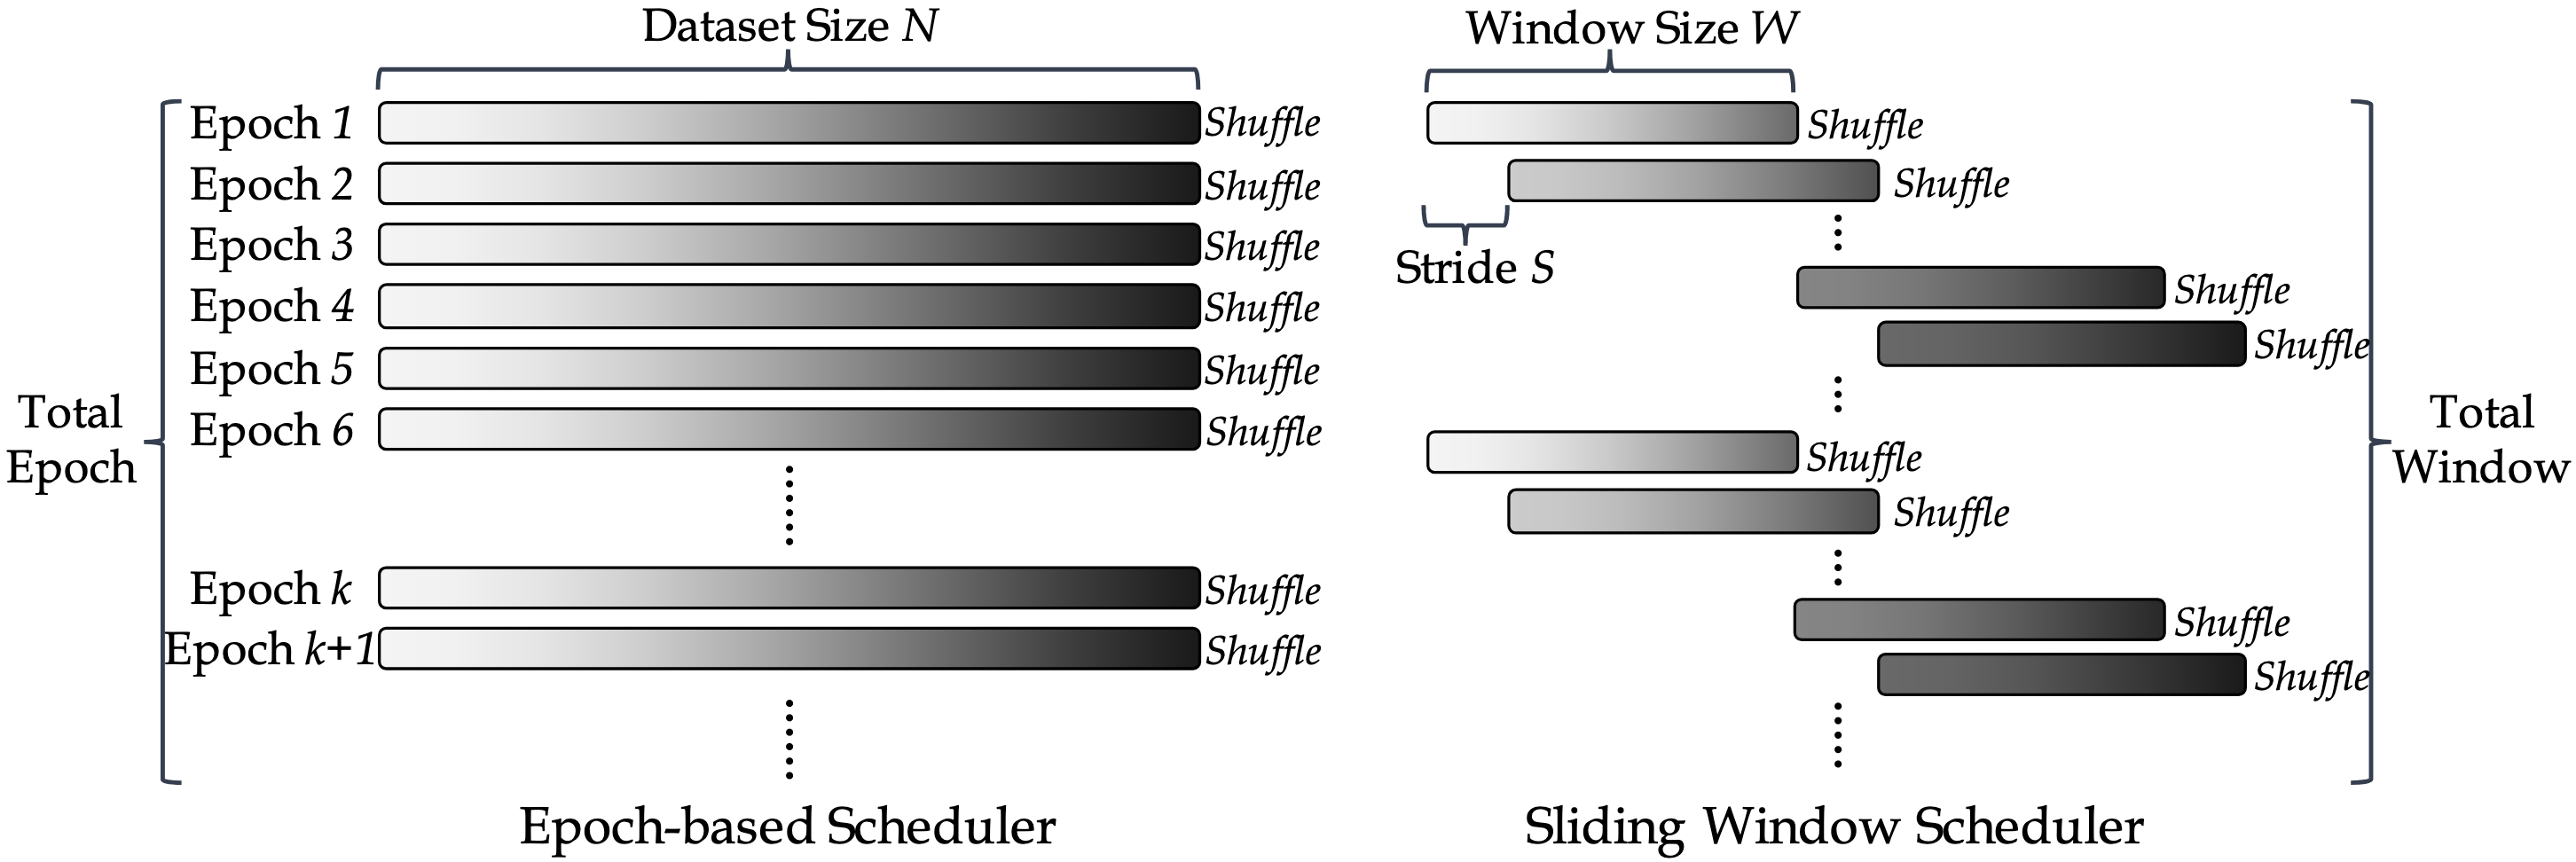
\includegraphics[width=300pt]{images/PIC_data_scheduler.png}
    \caption{Comparison of different data schedulers from \citet{PIC_2020}.
    While the epoch based version leads to long periods where instances are neglected in training,
    the sliding window approach ensures the majority of the instances are chosen more frequently.}
    \label{fig:pic_data_scheduler}
\end{figure}

% loss function
\citeauthor{PIC_2020} apply a cosine soft-max loss based on only the most recent $K$ instances 
to reduce computational costs.


\subsection{\acl{swav}}\label{subsec:SwAV}

\citet{swav_2020} proposed a novel approach to mine positive samples, called \ac{swav}.
It is an online clustering algorithm that works on batches of any size.
If the batch size $B$ is too small to form $K$ clusters the instances are augmented 
with instances from a previous batch, 
but only the original $B$ instances are considered in the loss function.
The approach forces the clusters to have roughly the same size, i.e. form an equipartition.

\citeauthor{swav_2020} claim their method needs neither a memory bank nor a momentum encoder.
The positive sample $x_{nt}$ for an instance $x_n$ is obtained by applying a 
random augmentation $t \in \mathcal{T}$ to $x_n$.
After embedding both the original and the augmented instance, clustering is performed and 
the loss function is computed as defined in \Eqref{eq:swav_loss}.
Opposed to other methods, this approach does not directly encourage similar embeddings but similar 
cluster assignments for positive pairs.
However, if both views are similarly encoded they should obtain the same cluster assignment.

\begin{equation}
    L(z_n, z_{nt}) = l(z_n, q_{nt}) + l(z_{nt}, q_n)
    \label{eq:swav_loss}
\end{equation}

The soft cluster assignments $q_n, q_{nt}$ for $x_n, x_{nt}$ respectively 
are used with the other instance's embedding to compute the loss.
The idea is to swap the assignments between the two views of the same image to encourage 
similar cluster assignments for similar instances as illustrated in \autoref{fig:swav_vs_cl}.
The loss $l(z_n, q_{nt})$ is a cross-entropy loss that uses the similarity between the prototype 
of the desired cluster and the embedding of the instance $z_n$ as the probability in the logarithm.

\begin{figure}[!htb] % h = here, t = top, b = bottom, p = page of floats
    \centering
    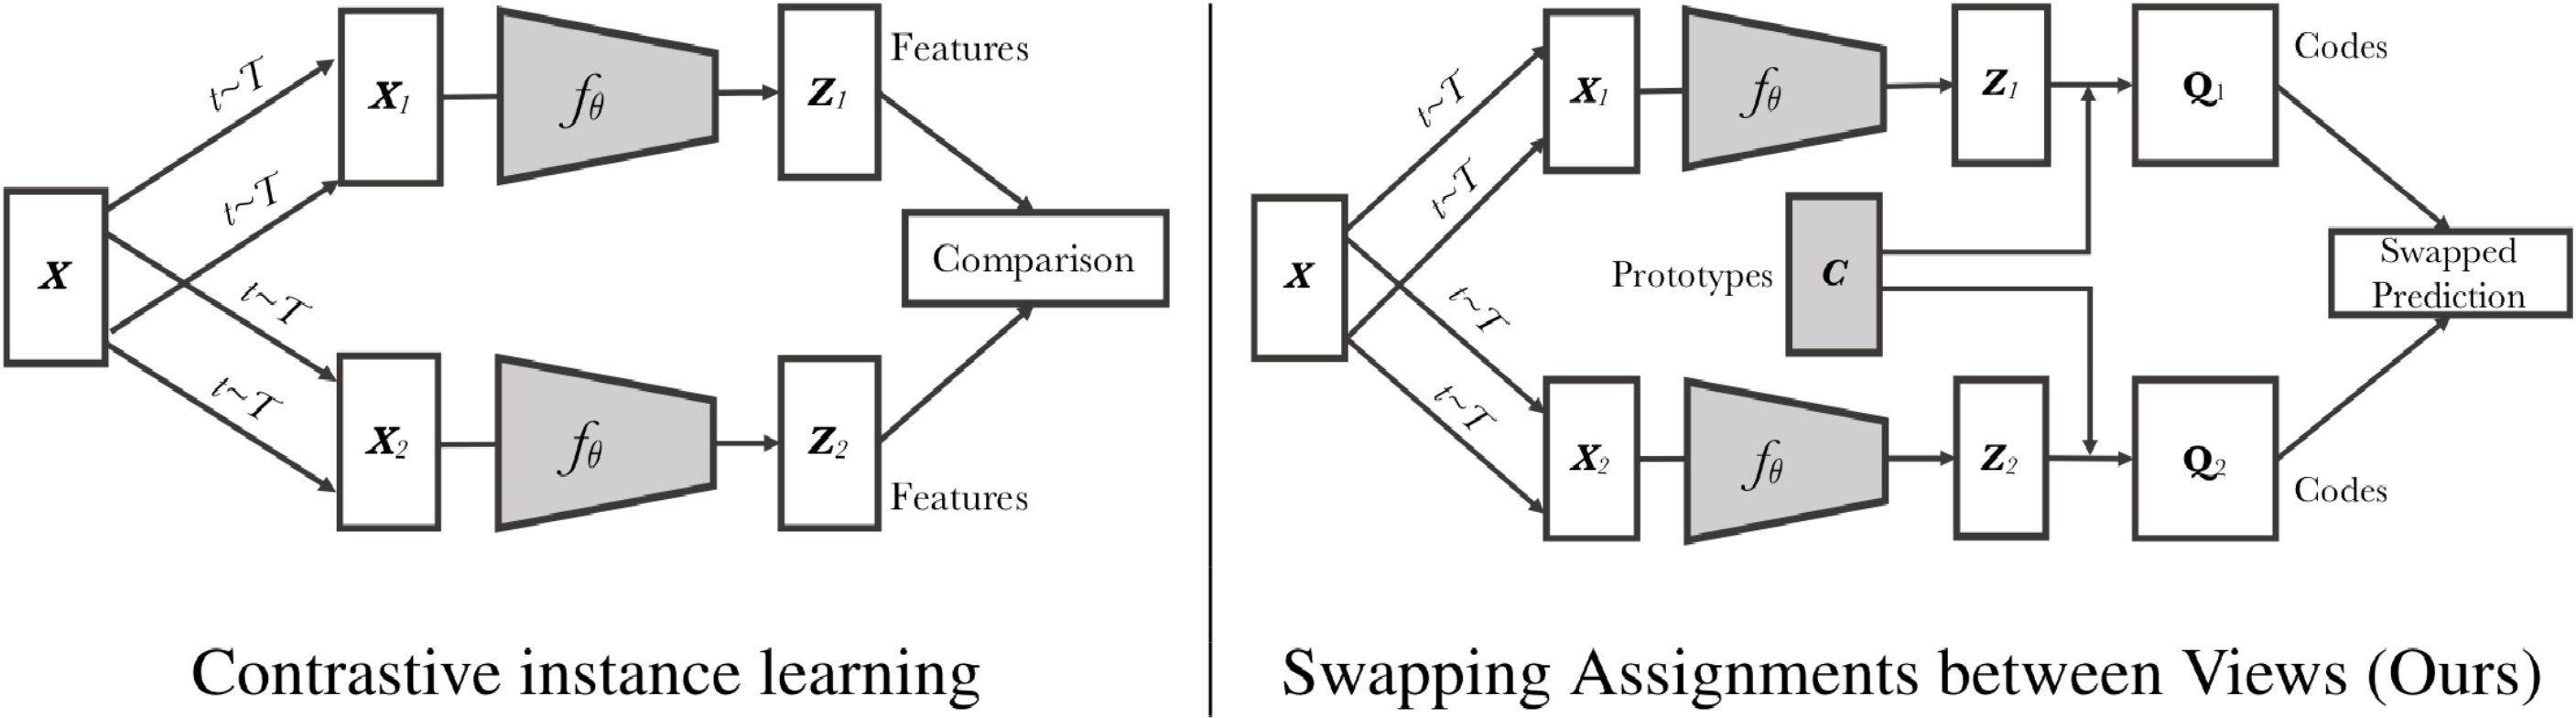
\includegraphics[width=300pt]{images/SwAV_vs_CL.png}
    \caption{Comparison of \ac{cl} and \ac{swav} from \citet{swav_2020}.
    \ac{cl} compares the augmented views directly while 
    \ac{swav} compares cluster assignments.
    Moreover, \ac{swav} computes the loss for an image and the cluster assignments of a positive augmentation 
    rather than its assignments and vice versa.}
    \label{fig:swav_vs_cl}
\end{figure}

\citeauthor{swav_2020} also introduce multi-crop, an augmentation technique that uses different 
crops of the same image.
They include two crops of standard size and standard resolution, 
and $V$ smaller size and low-resolution augmentations.
The resulting loss function is defined in \Eqref{eq:swav_loss_multicrop}.

\begin{equation}
    L(z_{t_{1}}, \cdots , z_{t_{V+2}})= \sum_{i\in \left\{ 1,2 \right\} }^{}\sum_{v=1}^{V+2} L_{v \neq i}(z_{t_{v}}, q_{t_{i}})
    \label{eq:swav_loss_multicrop}
\end{equation}

% end

% ---- Bibliography ----

% \bibliographystyle{splncs04}
\bibliographystyle{unsrtnat}
\bibliography{references}



\begin{acronym}

    \acro{nn}[NN]{Neural Network}
    \acro{cl}[CL]{Contrastive Learning}
    \acro{pu}[PU]{Positive-Unlabeled}
    \acro{fn}[FN]{False Negative}
    \acro{tn}[TN]{True Negative}
    \acro{ssl}[SSL]{Self-Supervised Learning}
    \acro{clae}[CLAE]{Contrastive Learning with Adversarial Examples}
    \acro{fgsm}[FGSM]{Fast Gradient Sign Method}

\end{acronym}

\end{document}
